%#######################################################################
%
% Introduction and motivation for open tool support and VDM + UML
%
\section{Introduction}
%-----------------------------------------------------------------------

%-----------------------------------------------------------------------
\subsection{Background}
%-----------------------------------------------------------------------

%
% Motivation
%
\frame
{
 \frametitle{Motivation}
%\begin{center}
  \begin{itemize}[<+->]
\itemsep=1cm
  \item<1-> Best of both by combining VDM and UML.
  \item<2-> Improve the limited tool support for VDM.
  \item<3-> Provide an easy to use and extensible user interface.
  \end{itemize}
%\end{center}
}

%
% Motivation combining knowlage
%
\frame
{
\frametitle{Communication}
  \begin{itemize}
	\itemsep=1cm
  		\item<1-> Formal Method (VDM)
  		\item<2-> Unified Modeling Language (UML)
  		\item<3-> Provide a brother platform of information sharing
  \end{itemize}

}

\note
{

  \begin{itemize}
	%\itemsep=1cm
  		\item Use a formal method to exactly specify what the system should do and prove that it does so.
  		\item Use UML to communicate to domain experts, thus a larger number of people can verify the model.
  		
  \end{itemize}



}

%
% Goal
%
\frame
{
  \frametitle{Goal}

\begin{center}

	\begin{block}<+->{Transformation}
	Provide a connection between VDM and UML. 
	\begin{itemize}
		\item Class Diagrams
		\item Sequence Diagrams
	\end{itemize}
	\end{block}
\vspace{1cm}
	\begin{block}<+->{Tool}
	Provide a open source easy to use extensible interface
	\begin{itemize}
		\item Availability
		\item Extendibility
	\end{itemize}
	\end{block}
%  \begin{itemize}
%	%\itemsep=1cm
%  		\item Provide a connection between VDM and UML
%  		\item Display a VDM static structure diagram (Class Diagram)
%  		\item Creation of Combinatorial Test statements from a dynamic diagram (Sequence Diagram)
%  		\item Integrate the transformation tool into Eclipse
%  		\item Open source
%	  	
%  \end{itemize}
\end{center}
}


%-----------------------------------------------------------------------
\subsection{Vienna Development Method}
%-----------------------------------------------------------------------
%
% VDM
%
\frame
{
  \frametitle{The Vienna Development Method}


  \begin{itemize}
	%\itemsep=1cm
  		\item<1-> VDM originates from Vienna in the 1970s
  		\item<2-> VDM Specification Language (VDM-SL) ISO released in '96
  		\item<3-> Extended in 1992-94 with object oriented structure and concurrency handling (VDM++).
  		\item<4-> Last extension made for distributed real-time systems (VICE).
  		\item<5-> Two most significant tool suites.
  		\begin{itemize}
  			\item VDM Tools - commercial
  			\item Overture - open source
  		\end{itemize}
	  	
  \end{itemize}


}

%
% Small VDM example
%
\frame
{
  \frametitle{VDM Train example}

\begin{center}

\vdmSpecLineNum{ClassDiagramOverview.vpp}{VDM classes with collections.}{VDM:Collections}

\end{center}
}

%-----------------------------------------------------------------------
\subsection{Unified Modeling Language}
%-----------------------------------------------------------------------
%
% UML
%
\frame
{
  \frametitle{Unified Modeling Language - UML}

	\begin{itemize}
	%\itemsep=1cm
  		\item<1-> UML is a semi-formal visual modeling language
  		\item<2-> Enabled developers to look at the system from different view points.
  		\item<3-> Comprised of differnt kinds of diagrams.
		\begin{itemize}
			%\item Primiary categoies of diagrams
			%\begin{itemize}
				\item Structure: Class Diagrams
				\item Behavior: Sequence Diagrams
			%\end{itemize}
		\end{itemize}
  		 
	  	
  \end{itemize}

}

\note
{
Used by developers to model a system at a desired levet of abstraction.



}


%
% Class Diagram
%
\frame
{
  \frametitle{Class Diagram}

\begin{center}

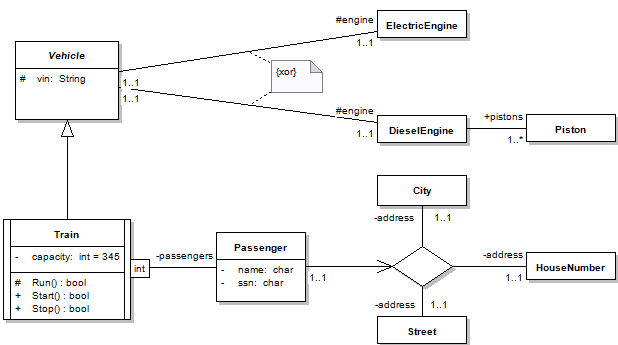
\includegraphics[width=\textwidth]{images/ClassDiagramOverview.png}

\end{center}
}

\note
{
\begin{itemize}
	\item Active class
	\item Generalization
	\item Visibility: public, proteted, private
	\item Association
	\begin{itemize}
		\item Qualified (int)
		\item N-ary
		\item Constraint (xor)
	\end{itemize}
\end{itemize}

}

%
% Sequence Diagram
%
\frame
{
  \frametitle{Sequence Diagram}

\begin{center}
	\includegraphics<1->[width=0.5\textwidth]{images/SequenceDiagram.png}%
\end{center}
}


\note
{
\begin{itemize}
	\item Life line
	\item Alternative: alt
	\item Loop
	\item Constraint
\end{itemize}

}
